\documentclass{standalone}
\usepackage{tikz}
\begin{document}
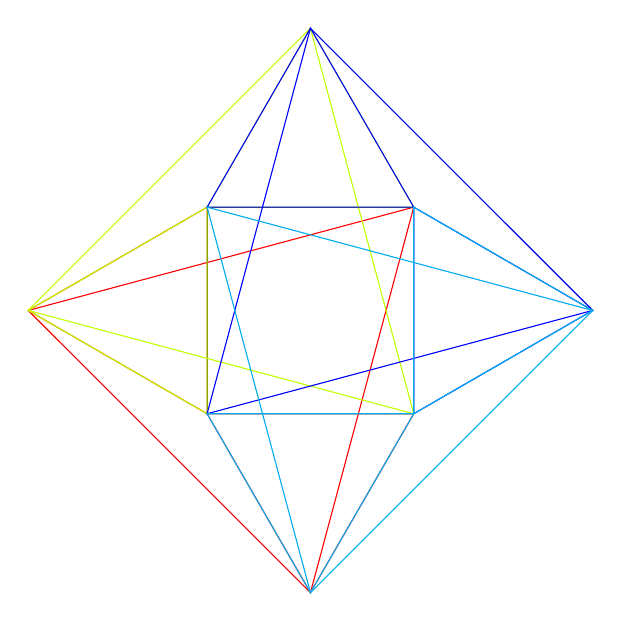
\begin{tikzpicture}[x=1pt,y=1pt]
\draw[red] (110.07,-165.66) -- (110.07,-91.00) -- (45.42,-128.33) -- cycle;
\draw[red] (184.72,-165.66) -- (110.06,-165.66) -- (147.39,-230.30) -- cycle;
\draw[red] (147.40,-230.30) -- (184.72,-91.01) -- (45.42,-128.33) -- cycle;
\draw (184.72,-91.00) -- (110.06,-91.00) -- (110.06,-165.66) -- (184.72,-165.66) -- cycle;
\draw[lime] (110.07,-91.00) -- (184.72,-91.00) -- (147.40,-26.35) -- cycle;
\draw[lime] (110.07,-165.66) -- (110.07,-91.00) -- (45.42,-128.33) -- cycle;
\draw[lime] (45.42,-128.33) -- (184.72,-165.66) -- (147.39,-26.36) -- cycle;
\draw[blue] (184.72,-91.00) -- (184.72,-165.66) -- (249.37,-128.33) -- cycle;
\draw[blue] (110.07,-91.00) -- (184.72,-91.00) -- (147.40,-26.35) -- cycle;
\draw[blue] (147.39,-26.35) -- (110.06,-165.65) -- (249.37,-128.32) -- cycle;
\draw[cyan] (184.72,-165.66) -- (110.06,-165.66) -- (147.39,-230.30) -- cycle;
\draw[cyan] (184.72,-91.00) -- (184.72,-165.66) -- (249.37,-128.33) -- cycle;
\draw[cyan] (249.37,-128.33) -- (110.07,-91.00) -- (147.40,-230.30) -- cycle;
\end{tikzpicture}
\end{document}
